\begin{flushright} {\tiny {\color{gray} (tikz\_P2.tex)}} \end{flushright}
%~~~~~~~~~~~~~~~~~~~~~~~~~~~~~~~~~~~~~~~~~~~~~~~~~~~~~~~~~~~~~~~~~~~~~~~~~~~~~~~~~~~~~~~~~~~~~~~~~~

\begin{center}
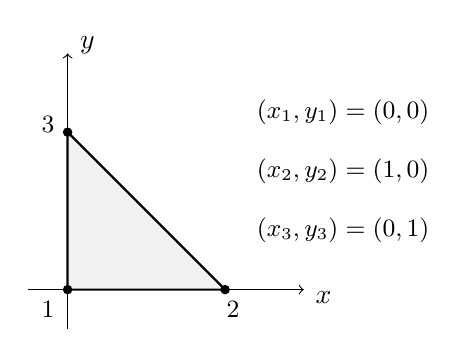
\begin{tikzpicture}
%\draw[step=0.5cm,gray,very thin] (0,0) grid (4,4); 
\draw[fill=gray!10,gray!10] (0.5,0.5)--(2.5,0.5)--(0.5,2.5)--cycle;
\draw[thick] (0.5,0.5)--(2.5,0.5)--(0.5,2.5)--cycle;
\draw [->] (0,0.5) -- (3.5,0.5);
\draw [->] (0.5,0) -- (0.5,3.5);
\node[] at (3.75,0.4) {$x$};
\node[] at (0.75,3.6) {$y$};
\draw[black,fill=black] (0.5,0.5)   circle (1.5pt);
\draw[black,fill=black] (2.5,0.5)   circle (1.5pt);
\draw[black,fill=black] (0.5,2.5)   circle (1.5pt);
\node[] at (0.25,0.25) {\small $1$};
\node[] at (2.6,0.25) {\small $2$};
\node[] at (0.25,2.6) {\small $3$};
\node[] at (4,2.75) {\small $(x_1,y_1)=(0,0)$};
\node[] at (4,2) {\small $(x_2,y_2)=(1,0)$};
\node[] at (4,1.25) {\small $(x_3,y_3)=(0,1)$};
\end{tikzpicture}
\end{center}

